% THIS IS AN EXAMPLE DOCUMENT FOR VLDB 2012
% based on ACM SIGPROC-SP.TEX VERSION 2.7
% Modified by  Gerald Weber <gerald@cs.auckland.ac.nz>
% Removed the requirement to include *bbl file in here. (AhmetSacan, Sep2012)
% Fixed the equation on page 3 to prevent line overflow. (AhmetSacan, Sep2012)

\documentclass{vldb}
\usepackage{graphicx}
\usepackage{balance}  % for  \balance command ON LAST PAGE  (only there!)
\usepackage{url}
\usepackage[utf8]{inputenc}
\usepackage{algorithm}
\usepackage{algpseudocode}
\usepackage{mathpartir}
\usepackage{amsfonts}
\usepackage{caption}
\usepackage{stmaryrd}
\usepackage{xcolor}


\newcommand{\es}{\texttt{ES}}
\newcommand{\txns}{$\Sigma$ }
\newcommand{\ex}{$\chi$}
\newcommand{\vis}{$\mathsf{vis}$}
\newcommand{\ar}{$\mathsf{ar}$}
\newcommand{\txno}{$\mathsf{txno}$}
\newcommand{\exo}{$\mathsf{exo}$}
\newcommand{\txn}{$\sigma$}


\newcommand{\mfalse}{\mathtt{false}}
\newcommand{\mtrue}{\mathtt{true}}
\newcommand{\mvis}{\mathsf{vis}}
\newcommand{\mar}{\mathsf{ar}}
\newcommand{\mtxno}{\mathsf{txno}}
\newcommand{\mwrio}{\mathsf{wrio}}
\newcommand{\mexo}{\mathsf{exo}}
\newcommand{\mex}{\chi}
\newcommand{\mtxns}{\Sigma}
\newcommand{\mtxn}{\sigma}
\newcommand{\mwri}{\texttt{wri}}
\newcommand{\Z}{\mathbb{Z}}
\newcommand{\fields}{\texttt{Fields}}
\newcommand{\recs}{\mathcal{R}}
\newcommand{\mevs}{\overset{\rightarrow s}{\mex}}
\newcommand{\mevsp}{\overset{\rightarrow s}{\mex_2}}
\newcommand{\mdang}{\mathtt{\zeta}}
\newcommand{\mrd}{\texttt{rd}}
\newcommand{\mcmd}{\mathsf{c}}
\newcommand{\select}{\mathtt{SELECT}}
\newcommand{\where}{\mathtt{WHERE}}
\newcommand{\stmt}[1]{\mathtt{Stmts}(#1)}

% Space in math mode
\newcommand {\myQQuad}[1] {\hskip#1\fontdimen6\font}


%% Inference Rules
\newcommand{\ALT}{~\mid~}
\newcommand{\RULE}[2]{\frac{\begin{array}{c}#1\end{array}}
                           {\begin{array}{c}#2\end{array}}}
\newcommand{\rulelabel}[1]{\textrm{\sc {#1}}}
\newcommand{\C}[1]{\texttt{#1}}
\newcommand{\F}[1]{\mathsf{#1}}
\newcommand{\M}[1]{\mathcal{#1}}


\newdef{definition}{Definition}
\newdef{theorem}{Theorem}


% Include information below and uncomment for camera ready
\vldbTitle{A Sample Proceedings of the VLDB Endowment Paper in LaTeX Format}
\vldbAuthors{Ben Trovato, G. K. M. Tobin, Lars Th{\sf{\o}}rv{$\ddot{\mbox{a}}$}ld, Lawrence P. Leipuner, Sean Fogarty, Charles Palmer, John Smith, Julius P.~Kumquat, and Ahmet Sacan}
\vldbDOI{https://doi.org/TBD}
\vldbVolume{12}
\vldbNumber{xxx}
\vldbYear{2019}


\begin{document}

% ****************** TITLE ****************************************

\title{A Sample {\ttlit Proceedings of the VLDB Endowment} Paper in LaTeX
Format\titlenote{for use with vldb.cls}}


% possible, but not really needed or used for PVLDB:
%\subtitle{[Extended Abstract]
%\titlenote{A full version of this paper is available as\textit{Author's Guide to Preparing ACM SIG Proceedings Using \LaTeX$2_\epsilon$\ and BibTeX} at \texttt{www.acm.org/eaddress.htm}}}

% ****************** AUTHORS **************************************

% You need the command \numberofauthors to handle the 'placement
% and alignment' of the authors beneath the title.
%
% For aesthetic reasons, we recommend 'three authors at a time'
% i.e. three 'name/affiliation blocks' be placed beneath the title.
%
% NOTE: You are NOT restricted in how many 'rows' of
% "name/affiliations" may appear. We just ask that you restrict
% the number of 'columns' to three.
%
% Because of the available 'opening page real-estate'
% we ask you to refrain from putting more than six authors
% (two rows with three columns) beneath the article title.
% More than six makes the first-page appear very cluttered indeed.
%
% Use the \alignauthor commands to handle the names
% and affiliations for an 'aesthetic maximum' of six authors.
% Add names, affiliations, addresses for
% the seventh etc. author(s) as the argument for the
% \additionalauthors command.
% These 'additional authors' will be output/set for you
% without further effort on your part as the last section in
% the body of your article BEFORE References or any Appendices.

\numberofauthors{3} %  in this sample file, there are a *total*
% of EIGHT authors. SIX appear on the 'first-page' (for formatting
% reasons) and the remaining two appear in the \additionalauthors section.

\author{
% You can go ahead and credit any number of authors here,
% e.g. one 'row of three' or two rows (consisting of one row of three
% and a second row of one, two or three).
%
% The command \alignauthor (no curly braces needed) should
% precede each author name, affiliation/snail-mail address and
% e-mail address. Additionally, tag each line of
% affiliation/address with \affaddr, and tag the
% e-mail address with \email.
%
% 1st. author
\alignauthor
Ben Trovato\titlenote{Dr.~Trovato insisted his name be first.}\\
       \affaddr{Institute for Clarity in Documentation}\\
       \affaddr{1932 Wallamaloo Lane}\\
       \affaddr{Wallamaloo, New Zealand}\\
       \email{trovato@corporation.com}
\alignauthor
G.K.M. Tobin\titlenote{The secretary disavows
any knowledge of this author's actions.}\\
       \affaddr{Institute for Clarity in Documentation}\\
       \affaddr{P.O. Box 1212}\\
       \affaddr{Dublin, Ohio 43017-6221}\\
       \email{webmaster@marysville-ohio.com}
\alignauthor
Ben Trovato\titlenote{Dr.~Trovato insisted his name be first.}\\
       \affaddr{Institute for Clarity in Documentation}\\
       \affaddr{1932 Wallamaloo Lane}\\
       \affaddr{Wallamaloo, New Zealand}\\
       \email{trovato@corporation.com}
\and \alignauthor
G.K.M. Tobin\titlenote{The secretary disavows
any knowledge of this author's actions.}\\
       \affaddr{Institute for Clarity in Documentation}\\
       \affaddr{P.O. Box 1212}\\
       \affaddr{Dublin, Ohio 43017-6221}\\
       \email{webmaster@marysville-ohio.com}
}
% There's nothing stopping you putting the seventh, eighth, etc.
% author on the opening page (as the 'third row') but we ask,
% for aesthetic reasons that you place these 'additional authors'
% in the \additional authors block, viz.
%\additionalauthors{}

\date{30 July 1999}
% Just remember to make sure that the TOTAL number of authors
% is the number that will appear on the first page PLUS the
% number that will appear in the \additionalauthors section.


%\maketitle
%\begin{abstract}
%\end{abstract}





%************************************************** 
\section{Introduction}
introduction


%************************************************** 
\section{Dependency graphs and serializability anomalies}
an overview of previous work on anomaly detection 

%************************************************** 
\section{Eventual Serializability}
In this section, we present the formal notion of \emph{Eventual
Serializability}, \es, and intuitively argue about its usefulness. Consequently, we
will introduce our ES anomaly detection algorithm as an extension to a previously known static
analysis technique \cite{Nagar:ser}. We will finally
present a handful of canonical examples from the literature and discuss how they all
implicitly conform to our notion of correctness.

\subsection {Definitions}
In this section, we assume (for the brevity of this
write-up) the SQL language and all definitions and operational rules from \cite{Nagar:ser}
are already presented to the readers. 

Given an abstract execution $ \mex = (\mtxns, \mvis, \mar)$, where \txns is a set of 
transaction instances, $\mvis \subseteq \mtxns \times \mtxns$ is an anti-symmetric, irreflexive relation
and $\mar \subseteq \mtxns \times \mtxns $ is a total, anti-symmetric
order on \txns such that $\mvis \subseteq \mar$, we define the \emph{write
set} of \txns as:
$ [\mtxns]_{\mwri} = \{\mwri(r,f,n) \;|\; \mtxn \vdash
  \mwri(r,f,n),\;
\mtxn \in \mtxns, n \in \Z, r \in \recs, f \in \fields  \} $, which is
the set of all writes to any field and record occured in any of the
executed transactions.

Assuming a total order of operations inside a transaction, \txno, and
a mapping \texttt{TXN()} from operations to their enclosing
transaction, we define a total order of writes within an execution as
follows: 
$$ w_1 \xrightarrow{\mwrio} w_2  \Leftrightarrow \texttt{TXN}(w_1)
\xrightarrow{\mar} \texttt{TXN}(w_2)  \vee w_1 \xrightarrow{\mtxno} w_2$$
We now define the \emph{eventual state} of the given execution,
denoted by $\mevs$, as the set of all writes performed on the database
and the absolute order between them, which is in accordance with the
fact that read operations do not affect the final state\footnote{read operations might 
affect writes indirectly by
providing them with values to be written; however, those values are already
captured in the write operations and it suffices to only include
write operations in our definition}. Formally:
  $$\mevs = ([\mtxns]_{\mwri},\mwrio) $$
Now we are ready to define \es, as our notion of application
correctness:

\begin{definition} 
  An abstract execution $ \mex_1 = (\mtxns, \mvis,\mar)$
  is said to be eventually serializable, if there exists another
  abstract execution $\mex_2$ which is serializable and has the same eventual state, i.e. 
  $\mex_2 \models \Psi_{Ser} $ and $\overset{\rightarrow s}{\mex_1}=
  \overset{\rightarrow s}{\mex_2}$.
\end{definition}
Note that $\mex_2$ in the above definition can theoretically include 
additional read-only transactions or altered transactions containing
additional read operations. However, since serializability is more
difficult to be achieved for executions with extra transactions or
operations, in order to prove a given execution eventually
serializable, the above definition intuitively guides us to first strip  certain
transactions and operations off the original execution and then prove
classic serializability for the trimmed execution.

\subsection {Dangling Reads}
In this part, we will introduce the notion of \emph{dangling reads}
as the ones whose sole purpose is to inform users about the current
state of the database, meaning that the values they return are not used anywhere in
the program (inside the following statements or path conditions). For example,
the \texttt{getBalance} transaction in a banking application contains a
single read operation on
the current balance of a given account, whose output is simply printed on the
user's screen but is not used anywhere else in the transaction.

We define a mapping $\mdang: \mrd \mapsto \texttt{bool}$, to keep
track of read operations that are dangling (which are mapped to
\texttt{false}). Such a mapping can be straightforwardly generated by a
static analysis of the input code
(similar to the dead-code-elimination step in any basic compiler) 
and in fact, we will present our
extended version of such an algorithm in the rest of this section.

Following \cite{Nagar:ser}, in order to detect eventual
serializability violations, we are going to build dependency graphs
form abstract executions and look for cycles. However, as we explained
above, certain operations are harmless against $\es$ and thus, cycles
containing such operations must be excluded from our analysis. 
We define a cycle $C$ to be \emph{effectful}, if and only if,
$\forall (r:\mrd) \in C.\; \zeta(r)$.

\begin{theorem}
  Given an abstract execution $ \mex = (\mtxns,\mvis,\mar)$, if there
  is no effectful cycle in the dependency graph $G_\mex$ then $\mex$ is
  eventually serializable.
\end{theorem}

\subsubsection{conditionally dangling reads}
The presented notion of dangling reads is already good enough to exclude many
practically harmless violations from our analysis; however, we can
further augment read operations with \emph{conditions} under which
they will become dangling. For example, consider the following transactions
(top)
in the dependency graph (bottom), from the courseware
application \cite{Gotsman:cise}: 
\begin{figure}[h]
  \begin{center}
    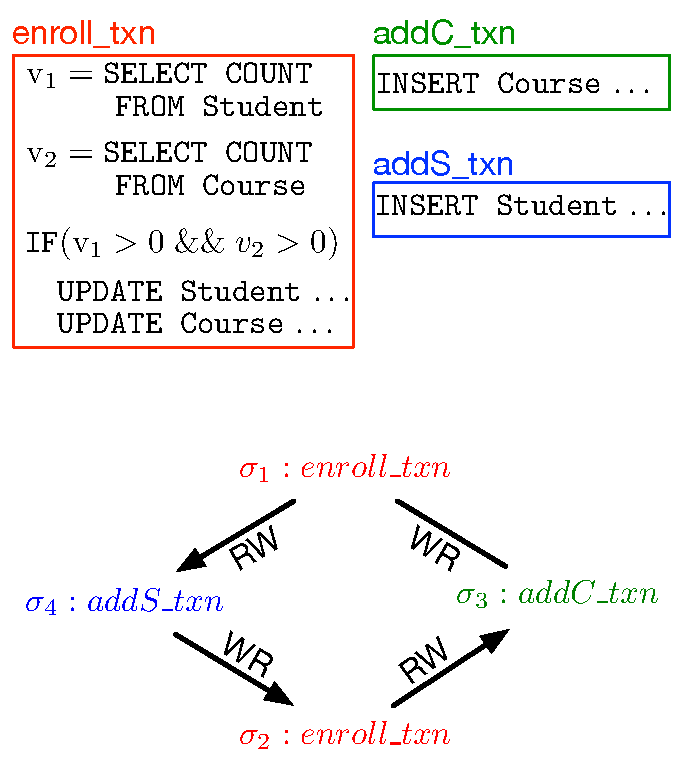
\includegraphics[scale=0.5]{figures/conditional_dangling.pdf}
  \end{center}
  \caption{a harmless violation}
  \label{fig:dangling}
\end{figure}

The situation in fig.\ref{fig:dangling} is clearly a violation of
classic serializability: $\sigma_1$ witnesses effects of
$\sigma_3$ but not $\sigma_4$ and $\sigma_2$ witnesses effects of
$\sigma_4$ but not $\sigma_3$, which creates a cycle as is depicted.
Moreover, a naive analysis looking for dangling reads would similarly
consider the given case a violation of \es, since values read by both reads
in enroll\_txn are used later inside the transaction and neither is seemingly
dangling. 

However, as acute readers may have noticed, 
the values read in enroll\_txn are subsequently used only under certain conditions.
In other words, the read operations can potentially become dangling
depending on the values they return. Following this observation, the
serializability violation in fig.\ref{fig:dangling} becomes harmless against $\es$ as the
guard ($v_1>0 \;\&\&\; v_2>0 $) can never be satisfied according to other
conditions present in the scenario.


Our goal in this paper, similar to \cite{Nagar:ser}, is to
construct a formula in FOL for a 
given transactional program $\mathbb{T}$ and a consistency
specification $\Psi$, such that any valid abstract execution
$\mex$ of $\mathbb{T}$ under $\Psi$ 
and its dependency
graph $G_\mex$ is a satisfying model of the formula. Consequently, we
can extend $\zeta$ to map each read operation to an FOL formula
(instead of a boolean), specifying the
conditions under which the read values become useful; 
these conditions
can be used later in our final formulation for a more accurate
analysis. 
As like before, $\mdang(\mrd)=\texttt{true}$ (never dangling) and 
$\mdang(\mrd)=\texttt{false}$ (always dangling) are the 
two extreme possible values of the map $\zeta$.

Before presenting our algorithm to statically construct $\zeta$
for a given transactional SQL program $\mathcal{T}$, we first define $\mathsf{src}(\mcmd)$ to be the set
of all read operations from which the values \emph{used} in $\mcmd$ are being sourced. 
Note that a value can be used in any statement and not just in writes, e.g. inside the 
$\where$ clause of a $\select$.
If the values used in $\mcmd$ are all constants or 
the input parameters of the transaction,
$\mathsf{src(\mcmd)}$ would trivially be empty\footnote{
we skip the formal algorithm for
 constructing $\mathsf{src(\mcmd)}$ in this paper,
as it is very straightforward using a simple data-flow analysis}.


\begin{algorithm}
\caption{Recursive construction of $\mdang$, given a transactional program $\mathcal{T}$, initially called with 
$\varphi = \texttt{true} $} \label{alg:dang} 

\begin{algorithmic}[1]
\Procedure{ExtractDanglig}{$\mcmd$,$\varphi$}
\State \textbf{match} $\mcmd$ \textbf{with}
\State \indent \textbf{case:} $\mcmd_1 \in \stmt{\mathcal{T}}$ 
\State \indent \indent \textbf{for} $\mrd$ \textbf{in} $\mathsf{src(\mcmd_1)}$ \textbf{do}
\State \indent \indent \indent $\mdang(\mrd)\gets \mdang(\mrd) \vee \varphi $
\State \indent \indent \textbf{end}

\State \indent \textbf{case:} $\mcmd_1;\mcmd_2$ 
\State \indent \indent \textsc{ExtractDanglig}($\mcmd_1$,$\varphi$)
\State \indent \indent \textsc{ExtractDanglig}($\mcmd_2$,$\varphi$)
\State \indent \textbf{case:} \texttt{IF} $\phi$ \texttt{THEN} \texttt{c}$_1$ \texttt{ELSE} \texttt{c}$_2$
\State \indent \indent \textsc{ExtractDanglig}($\mcmd_1$,$\varphi \wedge \phi$)
\State \indent \indent \textsc{ExtractDanglig}($\mcmd_2$,$\varphi \wedge \neg \phi$)
\State \indent \textbf{case:} \texttt{FOREACH} \texttt{v}$_1$ \texttt{IN} \texttt{v}$_2$ \texttt{DO} \texttt{c$_1$} \texttt{END}
\State \indent \indent \textsc{ExtractDanglig}($\mcmd_1$,$\varphi$)


\EndProcedure
\end{algorithmic}
\end{algorithm}



Assuming that $\mdang$ initially maps all read operations to $\mfalse$,
alg.\ref{alg:dang} recursively populates $\mdang$, constructing  a
map from each read operation in $\stmt{\mathcal{T}}$
to a formula made of the disjunction of \texttt{IF} conditionals enclosing
statements which are supplied by a value from that read.




\subsection{FOL Encoding}
In this section, we present our FOL encoding of transactional
program $\mathbb{T}$, as a formula parametric over a consistency specification $\Psi$, such
that any valid execution of $\mathbb{T}$ under $\Psi$ and its 
dependency graph is a satisfying model of the formula. We base our work on all of
the definitions and vocabulary from \cite{Nagar:ser} and present our slightly
modified version of their rules relating transactional programs to dependency
relations. 

As the result of choosing $\es$ as our notion of program correctness, which is weaker than classic
serializability, for each pair of transaction types $\mathcal{T}_1,\mathcal{T}_2
\in \mathbb{T}$ and a dependency type $\recs\in\{\mathsf{WR},\mathsf{RW}\}$,  we modified the 
rules populating $\eta^{\recs\rightarrow,\mathcal{T}_1,\mathcal{T}_2}_{} $ and 
$\eta^{\rightarrow\mathsf{WR},\mathcal{T}_1,\mathcal{T}_2}_{} $ (parametrized
over statements $\mcmd_1$ and $\mcmd_2$, exactly one of which must be a
\texttt{SELECT}), in a way to additionally
incorporate the conditions under which the \texttt{SELECT} statement is not
dangling. 
For example, our version of the rule that constructs the necessary entailments 
of an \textrm{RW} dependency relation is presented in the fig.\ref{fig:rwtus}:


\begin{figure}[h]
	\rulelabel{RW-Update-Select}
	$$
	\RULE
		{\mcmd_1 \equiv \tt{UPDATE\; SET}\; f = e_c\; \tt{WHERE}\; \phi_1 \\ 
		 \mcmd_2 \equiv \tt{SELECT} \; f \;\tt{AS}\; v\; \tt{WHERE}\; \phi_2 \\ 
		 \mcmd_1 \in  \C{Stmts}(\mathcal{T}_1) \quad \mcmd_2 \in  \C{Stmts}(\mathcal{T}_2) \quad \Gamma(t_1) = \mathcal{T}_1 \quad \Gamma(t_2) = \mathcal{T}_2}
		{ \eta_{\mcmd_2, \mcmd_1}^{\F{RW}\rightarrow,\mathcal{T}_2,\mathcal{T}_1}(t_2, t_1) =  
		 (\exists r.\ 
		 \mathcal{V}(\llbracket \Lambda_{\mathcal{T}_1}(\mcmd_1) \rrbracket_{t_1}) 
		  \wedge \mathcal{V}(\llbracket \phi_1 \rrbracket_{t_1, r} ) 
		 \; \wedge  \\ \myQQuad{5} \mathcal{V}(\llbracket  \Lambda_{\mathcal{T}_2}(\mcmd_2) \rrbracket_{t_2}) 
	    	\wedge \mathcal{V}(\llbracket \phi_2 \rrbracket_{t_2, r}) 
		 \; \wedge \\ \myQQuad{7}\C{Alive}(r, t_1)  \wedge \F{RW}(r, \F{f}, t_2, t_1)
 				\color{red} 
					\wedge \mathcal{V}(\llbracket  \zeta_{\mathcal{T}_2}(\mcmd_2) \rrbracket_{t_2}) 

 				\color{black})
	
}
	$$

\caption{a modified encoding rule}
\label{fig:rwtus}
\end{figure}






\subsection{Examples in the Literature}
to be done.



%************************************************** 
\section{ROT Extraction}
transaction chopping procedure. 

%************************************************** 
\section{Applicability and Prevalence}
review of all benchmarks verified and prevalence of extractable ROTs.

%************************************************** 
\section{Evaluation}
safety and performance evaluation

%************************************************** 
\section{Related Works}
detailed explanation please.

%************************************************** 
\section{Conclusions}
conclusions and future works

%************************************************** 









%\end{document}  % This is where a 'short' article might terminate

% ensure same length columns on last page (might need two sub-sequent latex runs)
%\balance

%ACKNOWLEDGMENTS are optional
%\section{Acknowledgments}

% The following two commands are all you need in the
% initial runs of your .tex file to
% produce the bibliography for the citations in your paper.
\bibliographystyle{abbrv}
\bibliography{../kia-bib}  % vldb_sample.bib is the name of the Bibliography in this case
% You must have a proper ".bib" file
%  and remember to run:
% latex bibtex latex latex
% to resolve all references

%\subsection{References}
%Generated by bibtex from your ~.bib file.  Run latex,
%then bibtex, then latex twice (to resolve references).

%APPENDIX is optional.
% ****************** APPENDIX **************************************
% Example of an appendix; typically would start on a new page
%pagebreak

%\begin{appendix}
%\section{Final Thoughts on Good Layout}
%\end{appendix}



\end{document}
